

\tikzset{every picture/.style={line width=0.75pt}} %set default line width to 0.75pt        

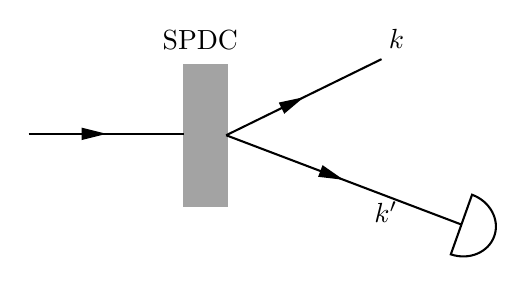
\begin{tikzpicture}[x=0.75pt,y=0.75pt,yscale=-1,xscale=1]
%uncomment if require: \path (0,300); %set diagram left start at 0, and has height of 300

%Shape: Rectangle [id:dp9291562475809372] 
\draw  [draw opacity=0][fill={rgb, 255:red, 0; green, 0; blue, 0 }  ,fill opacity=0.36 ] (144,109) -- (165.71,109) -- (165.71,177.67) -- (144,177.67) -- cycle ;
%Straight Lines [id:da8833130318893516] 
\draw    (69.71,142.67) -- (144.71,142.67) ;
\draw [shift={(107.21,142.67)}, rotate = 180] [fill={rgb, 255:red, 0; green, 0; blue, 0 }  ][line width=0.08]  [draw opacity=0] (12,-3) -- (0,0) -- (12,3) -- cycle    ;
%Straight Lines [id:da6688023135314647] 
\draw    (164.85,143.34) -- (239.71,106.67) ;
\draw [shift={(202.28,125.01)}, rotate = 513.9] [fill={rgb, 255:red, 0; green, 0; blue, 0 }  ][line width=0.08]  [draw opacity=0] (12,-3) -- (0,0) -- (12,3) -- cycle    ;
%Straight Lines [id:da8843982354889979] 
\draw    (164.85,143.34) -- (278,186.29) ;
\draw [shift={(221.43,164.81)}, rotate = 200.79] [fill={rgb, 255:red, 0; green, 0; blue, 0 }  ][line width=0.08]  [draw opacity=0] (12,-3) -- (0,0) -- (12,3) -- cycle    ;
%Shape: Chord [id:dp20648494743318113] 
\draw   (283.31,171.99) .. controls (291.94,175.15) and (296.75,183.92) .. (294.07,191.77) .. controls (291.36,199.74) and (281.96,203.75) .. (273.08,200.72) -- cycle ;

% Text Node
\draw (241.71,103.27) node [anchor=south west] [inner sep=0.75pt]    {$k$};
% Text Node
\draw (234.71,174.07) node [anchor=north west][inner sep=0.75pt]    {$k'$};
% Text Node
\draw (152.38,103.74) node [anchor=south] [inner sep=0.75pt]   [align=left] {SPDC};


\end{tikzpicture}
